\documentclass[output=paper]{langsci/langscibook} 
\ChapterDOI{10.5281/zenodo.1300614}
\author{Sofía Moratinos-Johnston\affiliation{University of the Balearic Islands }\and Maria Juan-Garau\affiliation{University of the Balearic Islands }\lastand Joana Salazar-Noguera\affiliation{University of the Balearic Islands }}
\title{The effects of English-medium instruction in higher education on students' perceived level and self-confidence in ELF}
\shorttitlerunninghead{The effects of English-medium instruction in higher education }
 

\abstract{Various studies (\citealt{Seikkula-Leino2007}; \citealt{Pihko2007}; \citealt{DoizEtAl2014clil}) carried out in secondary education have demonstrated the motivating effects of content-and-lan\-guage-integrated-learning (CLIL) programmes. However, they also indicate some problems with students’ self-concept in foreign languages caused by the difficulties encountered by learners. Compared with the sizeable number of studies focusing on CLIL and affective factors in secondary schools, there is still a lack of similar research at university level, where the term ‘Integrating Content and Language in Higher Education’ (ICLHE) is preferred. At this level students may have problems fully understanding lectures because of vocabulary difficulties or the lecturers’ pronunciation \citep{Hellekjaer2010}. In this study, we compare students’ linguistic self-confidence and perceived level of English according to the number of ICLHE subjects taken at university. Data was collected by means of a questionnaire administered to ICLHE students (n=155) and follow-up interviews (n=9). Results indicate a significant difference in participants’ level of linguistic self-confidence between those students that have taken one or two ICLHE subjects and those that have taken more than four. Similar results emerge as regards the students’ perceived level of English. These outcomes are corroborated by the interview data. They indicate that participants’ initial lack of self-confidence diminishes as students become accustomed to using English in their content classes, find strategies to cope with the challenges and start to intervene more. They also note an improvement in their level of English, which is translated into greater levels of enjoyment. The present study thus seems to imply that the more ICLHE courses taken, the better in terms of boosting linguistic self-confidence and perceived level of English.}
\maketitle

\begin{document}

 

\section{Introduction} 

The spread of courses ‘Integrating Content and Language in Higher Education’ (\isi{ICLHE}) taught in \ili{English} has been spurred by the fact that universities compete globally not only for international recognition, but also to attract foreign students and staff while promoting international research and networking (\citealt{Coleman2006}; \citealt{Graddol2006}; \citealt{Lasagabaster2015}; \citealt{Pérez-Vidal2015forall}). Other reasons include the promotion of \isi{multilingualism} in education driven by the European Union and the Council of Europe which results in the introduction of courses that integrate language and content at all levels of education (\cite{EuropeanHigherEducationArea2009}. However, although \isi{ICLHE} courses are becoming more and more common, differences can be noted in terms of their distribution across Europe. Whilst these courses are the norm in central and northern Europe, they are not so widely spread in southern Europe \citep{WächterMaiworm2014}, possibly due to the lower \isi{proficiency} levels found amongst university students and lecturers \citep{Cots2013,Arnó-MaciàMancho-Barés2015}. 



In Spain, \textit{Content and Language Integrated Learning} (\isi{CLIL}) was first implemented some two decades ago through a series of national and regional policies initiated in bilingual schools or the so-called ``European sections'' \citep{Cañado2010,Juan-GarauSalazar-Noguera2015}. Similarly, the \ili{Spanish} Ministry of Education recently introduced an initiative aimed at raising the international profile of \ili{Spanish} universities, whereby one out of three degree programmes will be taught in \ili{English} by 2020 (\citealt{SpanishMinistryofEducation2015}). 



The advantages for students associated with the inclusion of \isi{ICLHE} courses at university level are manifold, both academically and in terms of their future career development, be it locally or abroad. These advantages manifest themselves firstly as successful language \isi{acquisition}, as shown by many studies (e.g. \citealt{CoyleEtAl2010,RuizdeZarobe2011,Pérez-Vidal2013,Gené-GilEtAl2015}). However,  there are also some authors  (e.g. \citealt{Seikkula-Leino2007,Hunt2011,Bruton2013})  that argue that there may be a loss of self-esteem linked to the fact that students are required to use a language they do not really know for academic communication, resulting in decreased language use and demotivation, which may hamper language \isi{acquisition}. The fact that content is taught in a \isi{foreign language}, and that this language may be above the current competence of the student, makes \isi{ICLHE} a challenging endeavour requiring considerable effort and concentration on the students’ part. In the same vein, \citet{Hood2010} points out that, at the initial stages of instruction, enjoyment, motivation and self-esteem may suffer as students struggle to adapt to this new \isi{teaching approach}. Hence, \citet{CenozEtAl2014} suggest the need for more research on some of these still unanswered questions. It is therefore worth investigating at what stage students start to feel more comfortable in their \isi{ICLHE} classes. With this goal in mind, this study explores:


\begin{itemize}
\item students’ \isi{linguistic} self-confidence and perceived level of \ili{English} according to the number of \isi{ICLHE} subjects taken at university
\item the reasons for any initial lack of confidence in their abilities
\item the strategies that learners use to cope with the challenges.
\end{itemize}

\section{Literature review}


{Linguistic self-confidence and self-perception of \isi{L2} achievement}

Delving into the historical development of \isi{L2} motivational research (\citealt{DörnyeiUshioda2011}), we find that during the \textit{social psychological period} (1959-1990) \citet{GardnerLambert1959} pointed out  that there seemed to  be  two main factors affecting \isi{L2} achievement: language aptitude and a group of attitudinal and motivational variables that they referred to as the motivation factor. As a matter of fact, \citegen{Gardner1985} most well-known contribution to the development of motivation research, the \textit{\isi{socio-educational model},} aimed at explaining how these attitudinal and motivational components fostered second language \isi{acquisition} (\isi{SLA}). The relationship between motivation and \textit{orientation} is a key feature in this model, which distinguishes between \textit{integrative} and \textit{instrumental orientations.} 



A significant finding was the important role that the self-perception of \isi{L2} achievement played in successful \isi{SLA}. These studies suggested that \isi{proficiency} in \ili{English} was associated with a concept that was labelled as ‘Self-Confidence with \ili{English}’. Students with high self-confidence:


\begin{quote}
experienced little anxiety when speaking \ili{English} in class or in real life situations, perceived themselves as being competent in their \ili{English} abilities, reported frequent use of \ili{English}, had positive attitudes towards their \ili{English} class, showed motivation and desire to learn \ili{English}, had experiences with more than one language at home, and performed well on indices of achievement in \ili{English}. \citep[24]{SampasivamClément2014}
\end{quote}



A strand within Gardner’s \textit{socio-educational model}, the \textit{socio-contextual model,} proposed by \citet{Clément1980}, accounted for the above-mentioned findings and first developed the concept of ‘\textit{\isi{linguistic} self-confidence}’, which was defined by social contact with the \isi{L2} group and modulated by its  frequency and its quality. Thus, although the concept of \isi{linguistic} self-confidence is largely defined socially, particularly within \isi{multilingual} communities, it also has a cognitive component - ‘the perceived \isi{L2} \isi{proficiency}’. The more positive our self-perceived \isi{proficiency} and the lower our anxiety levels, the higher our levels of \isi{linguistic} self-confidence will be. Linguistic self-confidence also greatly influences the willingness to communicate (WTC) in the \isi{foreign language classroom} \citep{MacIntyre1EtAl998}.  For instance some studies in Asia indicate that, apart from cultural factors, individual factors such as self-confidence play an important role in classroom situations that demand interaction such as group tasks \citep{ShaoGao2016,Eddy-U2015,Yashima2002}. Again in a classroom environment, \citet{Dörnyei2001} drew up a list of nine demotivating factors linked to a total of 75 occurrences, 11 of which  were related to reduced self-confidence following a negative experience in class. There also seem to be differences in perceived self-confidence according to the level of \isi{proficiency}. Lower \isi{proficiency} learners feel demotivated earlier during their learning experience and blame internal factors such as unsatisfactory performance or reduced self-confidence, while higher \isi{proficiency} learners tend to blame the teachers \citep{FaloutMaruyama2004}. 



While \isi{linguistic} self-confidence is thought to have a positive effect on \isi{SLA} and motivation \citep{Dörnyei2005}, its opposite,  ‘anxiety’, has a mostly negative effect. \citet[284]{MacIntyreEtAl1994} define it as ‘the feelings of tension and apprehension specifically associated with second language contexts’. \citet{HorwitzEtAl1986} refer to the \isi{foreign language classroom} environment as a context where learners are very likely to have difficulty understanding others and making themselves understood. Research shows that the effects of foreign \isi{language anxiety} on the learner include forgetting previously learned material, decreased participation, negativity and avoidance behaviour (\citealt{GregersenHorwitz2002}). Consequently, learners will only be confident in their \isi{linguistic} abilities if they lack anxiety and have positive feelings about their \isi{proficiency} in the \isi{L2}. \citet{SampasivamClément2014} have put together a model describing the relationship between a number of factors that determine \isi{L2} confidence. At the centre of the model are richness and self-involvement. Richness refers to the various channels through which we receive the \isi{L2} input, which should be varied in form and allow for feedback to be effective. The fact that we are able to understand this \isi{rich input} positively affects self-confidence, while self-involvement is related to the level of interaction that learners maintain in response to this input. \citet{Yashima2002} claims that self-involvement is in turn shaped by the perceived importance of the contact experience and gives an example of this relationship which is related to the concept of \textit{international posture}. People who value international communication are more likely to place more value on this type of contact experiences and be therefore more motivated to learn the \isi{L2}, which in turn results in higher levels of \isi{L2} confidence \citep{Yashima2009}. 



The relationship between richness and \isi{L2} confidence is mediated by two variables: (1) frequency of contact; and (2) \isi{proficiency}.  An increased frequency of contact, even when low in richness, is expected to lead to an increase in \isi{L2} confidence. Similarly, \isi{proficiency} is also associated with \isi{L2} confidence.  Learners with adequate levels of \isi{proficiency} are less likely to be overwhelmed by \isi{rich input}, experiencing greater levels of satisfaction and confidence while beginners can suffer  from anxiety if they are exposed to rich forms of contact \cite{OzdenerSatar2008}.



The last variable described in \citegen{SampasivamClément2014} model is \textit{quality}, which influences the relationship between self-involvement and \isi{L2} confidence. This variable refers to the pleasantness of the contact experience and how it positively or negatively affects self-confidence. 



Since \isi{linguistic} self-confidence and the self-perception of \isi{L2} achievement are thought to play an important role as regards motivation, WTC and subsequent \isi{SLA}, these are variables worth considering when researching how the introduction of a \isi{teaching approach} such as \isi{ICLHE} affects the learners. More specifically, as this approach is supposed to foster interaction between teacher and learners and the learners themselves \citep{Coyle2007},  WTC will become especially important in these classes.  Moreover, \isi{ICLHE} is also known to be cognitively demanding \citep{CoyleEtAl2009} and therefore may affect each learner’s self-esteem differently. In the next section, we will look at the nature of these challenges, their consequences and how the students tackle the difficulties they may encounter. 


\section{Content and language integration: the challenges, students’ responses and the effects of increasing exposure to ICLHE} 
 

The \isi{sociocultural} tenet that language use mediates language learning   \citep{Swain2000output}  in an \isi{ICLHE} context implies ‘a level of talking, of interaction and dialogic activity which may be different to that of the traditional language or content classroom’ \citep[554]{Coyle2007}. Moreover, if the content is conceptually difficult, the added hurdle of the \isi{foreign language} may make it even more difficult for students to assimilate both language and content simultaneously (\citealt{Seikkula-Leino2007}). Some students may feel that they are expected to perform at a more advanced level than that which they consider realistically possible, resulting in a decreased lack of confidence, despite the improvement in their grades. There may be therefore a discrepancy between the progress revealed by formal assessment and the students’ own perception of progress \citep{Mearns2012}. If we now turn to the \isi{CLIL} contexts, their demanding nature requires higher levels of concentration amongst students, who may perceive this as too much of an imposition \citep{Hunt2011} and feel more anxious,  as  \citet{SylvénThompson2015} and \citet{SantosMenezesJuanGarau2013} confirmed.  These studies were undertaken in secondary schools at initial stages of \isi{CLIL} implementation, when students had not yet had much exposure to this new \isi{teaching approach}.  However, as exposure increases by the third grade of secondary education, differences between \isi{CLIL} and non-\isi{CLIL} students’ anxiety levels seemed to decrease, as \citegen{DoizEtAl2014clil} study reveals.



As regards \isi{ICLHE} research in Spain, \citet{Arnó-MaciàMancho-Barés2015} and \citet{Breeze2014} discovered that  \isi{ICLHE} students were very aware of their low language \isi{proficiency} level, including problems of comprehension and their inability to express complex content knowledge in a \isi{foreign language} \citep{Muñoz2001,FeixasEtAl2009}. Nevertheless, \citegen{AguilarRodríguez2012} study,  targeting engineering students, reported  satisfactory results in terms of vocabulary \isi{acquisition} and listening skills, despite objections to the lecturer’s level of \ili{English}. It is precisely lecture comprehension, a skill that seems hard to master in \isi{ICLHE} classes, which worries students. For example,    \citet{FlowerdewMiller1992} discovered that some of the areas that students identified as difficult were handling the speed of lecture delivery, understanding new terminology and concepts and concentrating during extended periods of time. In Norway, \citet{Hellekjaer2010} described difficulties understanding certain parts of the lecture because of unclear \isi{pronunciation}, unknown vocabulary and difficulty taking notes. To all this \citet{Breeze2014} added the high speed of delivery of lectures, which hinders comprehension. Finally, students also appreciated a clearer structure in lecture organization as Dafouz and Núñez (\citeyear{DafouzNúñez2010}) pointed out. Although switching to a \isi{foreign language} can have an initial negative effect that may adversely affect university students’ grades, \citet{Klaassen2001} found that differences in grades between students following \isi{ICLHE} and traditional teaching methods were no longer noticeable after one year.  The students had adapted to the language change thanks to a number of strategies that helped compensate for these negative effects. The strategies students used to overcome their language problems included: looking up difficult words and L1 use (see also \citealt{Coonan2007}); researching the subject both before and after the lecture; relying on peers and teachers or tutors for help, and trying to improve their concentration skills (\citealt{FlowerdewMiller1992}).   \citet{AireyLinder2007} found that some students would concentrate on taking notes instead of focusing on the contents. The solution in this case was to stop taking notes and read the textbook or class materials before the lecture instead. 



To conclude, over the years there have been various studies analysing the impact of  \isi{ICLHE} courses, focusing on their effect on the students and the  many challenges these have to face (e.g. \citealt{Arnó-MaciàMancho-Barés2015,AguilarMuñoz2014}). We believe that more research is needed on the latter aspect, including analysing the point at which these challenges and their effects on students’ \isi{linguistic} self-confidence start to recede as a consequence of their increased exposure to \isi{ICLHE} courses. These issues will be analysed in this study along with the strategies students use to overcome the difficulties they face, with a view to helping other students who are uncertain about their \isi{linguistic} abilities.


\section{The present study}

The research questions that this study intends to answer are the following:


\begin{itemize}
 \item [\textbf{RQ1.}] At what stage do \isi{ICLHE} students start to build up \isi{linguistic} self-confi\-dence and perceive an improvement in their level of \ili{English}?
\item [\textbf{RQ2.}] Why do some \isi{ICLHE} students display an initial lack of self-confidence and what strategies do these students use to overcome the difficulties they face?
\end{itemize}






\section{Method} 

\subsection{The study’s design, setting and sampling decisions}

Our study forms part of a larger project that examines motivation in different language learning contexts: Formal Instruction (\isi{FI}), \isi{ICLHE} and \isi{Study Abroad} (SA) (\cite{MoratinosJohnstonForthcoming}). Within this project, we decided to focus specifically on students that had experienced \isi{ICLHE} subjects, since the literature review had revealed the potential detrimental effects on their \isi{linguistic} self-confidence caused by the challenges associated with simultaneous content and language learning. 



Our study targets undergraduate students in the University of the Balearic Islands, a university which is also involved in a process of \isi{internationalization} aiming to attract foreign students.  In terms of the number of subjects taught in \ili{English}, the degree that offers the most is obviously the \ili{English} major degree. As for other degrees, the number varies according to the faculty and department policy. Some faculties, such as Tourism or Business and Economics, offer an optional pathway in \ili{English}. For example, the Tourism Faculty requires students following the pathway to take 30 mandatory ECTS in \ili{English}, study abroad for at least one semester and write a dissertation in \ili{English}. The requirements in the Business and Economics Faculty are similar yet more demanding since students have to take at least 100 ECTS of the degree in \ili{English}. Apart from all these \isi{ICLHE} subjects offered on Tourism and Business and Economics degree courses, other degrees also offer a much smaller amount of \isi{ICLHE} subjects, ranging from nine in the case of the Law degree to two in the case of Biochemistry. Considering that one of the aims of this study was to target students who had experienced \isi{ICLHE}, the sampling technique chosen was \textit{stratified random sampling} where ‘the population is divided into groups or \textit{strata} and a random sample of proportionate size is selected from each group’ \citep[97]{Dörnyei2007}. The stratification variables used were the different subject areas present in the university, which allowed us to include a higher proportion of students from the Tourism, Social Sciences and Law degrees, since these are the most popular degree courses.



A smaller sample was extracted, in order to carry out in-depth interviews. Participants were selected based on the results of a questionnaire (see for a detailed description 4.3 below). Since we were interested in obtaining a diverse sample, reflecting various levels of \isi{linguistic} self-confidence, we looked at the participants’ scores on this scale in the questionnaire, together with the number of \isi{ICLHE} subjects they had taken. Nine students that showed a high variance on these measures and in \isi{L2} \isi{proficiency} levels were thus selected. 


\subsection{Participants}

In the present study, we analysed the data from a group of students (n=155) from the University of the Balearic Islands in Spain. The overall majority of these students know \ili{Catalan} and \ili{Spanish}, the two official languages in the region, \ili{Catalan} being the local and \ili{Spanish} the state language. 



\tabref{tab:moratinos:1} presents an overview of the participants' main characteristics and the number of \isi{ICLHE} subjects they took. These students were in their first (N=51), second (N=33), third (N=28) and fourth (N=43) year of their studies and the majority were between 18 and 22 years of age. 


\begin{table}
\caption{Characteristics of the sample and number of ICLHE subjects taken}
\label{tab:moratinos:1}

\begin{tabularx}{\textwidth}{lQrr}
\lsptoprule
\multicolumn{3}{l}{\textbf{General information} } & \\
 \midrule
 \textbf{Sex}  & Female & 94 & 60.6\%\\
& Male & 61 & 39.4\%\\
\tablevspace
 \textbf{Studies}  & Tourism & 74 & 47.7\%\\
& Modern languages & 24 & 15.4\%\\
& History & 18 & 11.6\%\\
& Primary Education & 17 & 10.9\%\\
& Business and Economics & 12 & 7.8\%\\
& Engineering and Science\par & 10 & 6.6\%\\
 \textbf{ICLHE}  & 1 subject & 54 & 34.8\%\\
& 2 subjects & 23 & 14.8\%\\
& 3 subjects & 24 & 15.5\%\\
& 4 subjects & 4 & 2.6\%\\
& > 4 subjects & 50 & 32.3\%\\
\lspbottomrule
\end{tabularx}
\end{table}

More than half of the students (66.9\%) declared that they had an intermediate level of \ili{English} (B1/B2), as shown in Figure 1. Amongst them, one third of the participants (35.1\%) declared they had a B2, the minimum level of listening ability that \citet{Breeze2014} recommends before one begins an \isi{ICLHE} course, while (20.7\%) stated that they had a C1 level or above, which probably means that these students could feel at ease and possibly learn more in their classes. The remaining students’ (12.4\%) perceived level ranged between a B1 to basic level (A1/A2) or non-existent. 


\begin{figure}
% 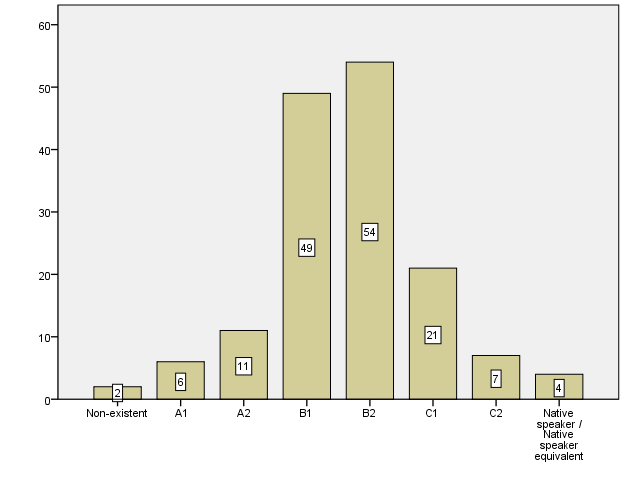
\includegraphics[width=\textwidth]{figures/moratinos-img1.png}
\barplot{level}{\%}{non-existent,A1,A2,B1,B2,C1,C2,NS/NSE}{
  (non-existent,2)
  (A1,6)
  (A2,11)
  (B1,49)
  (B2,54)
  (C1,21)
  (C2,7)
  (NS/NSE,4)
}
\caption{Perceived level of English of the participants. NS(E)= native speaker (equivalent).} 
\label{fig:moratinos:1}
\end{figure}


   
 



Interviewees (n=9) were balanced for gender and came from a varied range of degree courses where \isi{ICLHE} subjects were offered, as seen in Table 2 below. 


\begin{table}
\caption{Characteristics of the interviewees}
\label{tab:moratinos:2}

\begin{tabularx}{\textwidth}{lllrSS}
\lsptoprule
 Initials & Gender & Degree & Year & No. \isi{ICLHE} subjects & Perceived level of \ili{English}\\
 \midrule
 MG & male & Economics & 2 & 2 & C1\\
 MV & male & \ili{Catalan} & 1 & 1 & A2\\
 MJG & female & Tourism & 3 & >4 & B1\\
 DM & male & Tourism & 1 & 3 & B1\\
 MFS & female & \ili{English} & 4 & >4 & C1\\
 LM & female & \ili{English} & 4 & >4 & C2\\
 VC & female & History & 1 & 1 & A2\\
 \isi{IM} & male & History & 1 & 1 & A2\\
 IR & male & History & 1 & 1 & B2\\
\lspbottomrule
\end{tabularx}
\end{table}

\subsection{Instruments}

A mixed-method approach was followed, as it offers the advantages of triangulation, complementarity and cross-validation of the findings (\citealt{IvankovaGreer2015}). Thus, two research instruments were used in our study, a questionnaire and interviews. 


\newpage 
The questionnaire used in the survey was developed following \citegen{Dörnyei2010} guidelines, and comprised two parts: the first consisted of 19 questions designed to establish the participants’ \isi{linguistic} profile (e.g. mother tongue and self-rated \ili{English} \isi{proficiency} level) and the types of language \isi{learning context} experienced (\isi{FI}, \isi{CLIL} and SA), while the second part included 47 six-point Likert-type items (ranging from strongly disagree to strongly agree). These items were adapted from three previously published motivation questionnaires: \cite{CsizérKormos2009} Motivation Questionnaire for College and University Students in Hungary, \citegen{TaguchiEtAl2009} motivation questionnaires and \citegen{Ryan2009} Motivation Factors Questionnaire. The items were translated and modified (where necessary) to suit the \ili{Spanish} cultural context. The administration procedure involved first contacting UIB lecturers, whose \isi{ICLHE} courses had been selected on a random basis. These lecturers then informed their students that a questionnaire would be administered to all those wishing to participate. On each occasion, the administrator (i.e. the first author of this paper) introduced the questionnaire which took on average 15 minutes to fill in. Response rates were high (over 98\%).



In this study, we will focus on the findings revealed by the questionnaire as regards the two variables under scrutiny – the perceived level of \ili{English} of the participants and their \isi{linguistic} self-confidence as described below:


\begin{itemize}
\item Perceived level of \ili{English}:  participants rated themselves by choosing one of seven CEFR levels ranging from non-existent to \isi{native speaker}/native speaker-like. 
\item Linguistic self-confidence (5 items adapted from \citegen{Ryan2009} questionnaire): measuring the level of confidence that the participants had in their abilities as \isi{L2} learners and users. The items, three of which were negatively worded, were the following:

\begin{enumerate}
\item I am sure I am able to learn a \isi{foreign language}.
\item I worry that other students will laugh at me when I speak \ili{English}. 
\item Learning a \isi{foreign language} is easy for me. 
\item I think I am the type who would feel anxious and ill at ease if I had to speak to someone in a \isi{foreign language}. 
\item I always think that my classmates speak \ili{English} better than I do. 
\end{enumerate}
\end{itemize}

The \isi{linguistic} self-confidence scale was found to have a high internal consistency (Cronbach’s alpha = .78). 



Interviews were an additional instrument of this study. They were used to further interpret the findings revealed by the questionnaire data. Thus, the larger scale perspective was enriched by personal exchanges with the participants, following a model that \citet[170]{Dörnyei2007} describes as ‘questionnaire survey with follow-up interviews or retrospection’. This approach allows us to interpret unexpected results that may arise from the data by inviting the participants to explain them individually. In addition, the interviews became narrative accounts of the participants’ language \isi{learning history}. The learners’ accounts described how they felt throughout different stages across microlevel timescales (\citealt{MercerWilliams2014}). Interviews also allowed the participants to point out and develop those factors that they themselves found the most relevant to their \isi{learning history}. 



The semi-structured interviews with set questions aimed at exploring:


\begin{itemize}
\item the participants’ feelings at the time of their lessons,
\item their language simultaneously,
\item strategies used to overcome potential learning difficulties,
\item their overall evaluation of the course (including the teacher, their peers, materials, impressions of their level of \ili{English} and the fact that they were learning content and etc.).
\end{itemize}

These questions allowed us to investigate a wider topic area, resulting in nine in-depth narrative interviews in the participants’ mother tongue, which lasted between 60 and 90 minutes. Participants’ quotations are reported using an identification code, which includes the initials of their first and last name. After obtaining the participants’ consent, all interviews were audio recorded and fully transcribed following \cite{Richards2003} recommendations. Excerpts presented in this study were translated from \ili{Catalan} or \ili{Spanish} into \ili{English} by the interviewer.


\subsection{Data analysis}

The questionnaire was piloted and went through reliability analysis by means of principal component analysis using SPSS 22. We then carried out normality tests, which showed the normality of the data, allowing us to use parametric tests. 



The interviews were coded according to emerging themes, patterns or conceptual categories that helped structure the data in order to discover the wider picture developing from some of these recurring themes \citep{Saldaña2013}. The conceptual categories in the  theoretical framework on \isi{L2} confidence  developed by \citet{SampasivamClément2014} were used as the basis for  analysis. The goal was to identify the links between the recurrent themes and these conceptual constructs \citep{Pavlenko2007}, yet also keeping an open mind for possible unexpected themes that might have appeared. The coding process was done using NVIVO 11.


\section{Results and discussion}


\subsection{RQ1. Linguistic self-confidence and perceived level of English according to ICLHE subjects taken}

In order to answer the first \isi{research question}, we analysed whether there were any statistical differences between the participants as regards their levels of \isi{linguistic} self-confidence and perceived level of \ili{English} according to the number of \isi{ICLHE} subjects taken using a one-way between groups ANOVA. 



The results revealed that there was a statistical difference in terms of \isi{linguistic} self-confidence F (4, 154) = 3.98, (p =.004) between the groups of participants divided according to the number of \isi{ICLHE} subjects taken. The effect size, calculated using eta squared, was .09, which according to \citet{Cohen1988} is considered a medium effect size.  \textit{Post hoc} comparisons with Tukey HSD indicated that the mean score for the students that had taken one (M=4.22) and two \isi{ICLHE} subjects (M=3.92) were lower and significantly different from the group of students that had taken more than four subjects (M=4.76), who had higher levels of \isi{linguistic} self-confidence on the six-point scale, as seen in Table 3. There were no statistically significant differences amongst the other groups. However, although the difference was only statistically significant after taking more than four \isi{ICLHE} subjects, having done three subjects (M=4.61) already helped to improve the students’ self-confidence. These findings are in line with \cite{DoizEtAl2014clil} study that noticed a decrease in levels of anxiety in the third grade of secondary education as students progressed in their studies and became used to instruction in \ili{English}.  Furthermore, they confirm that the more frequent the contact with \isi{rich input}, such as after taking multiple \isi{ICLHE} classes, the higher the \isi{L2} confidence \citep{SampasivamClément2014}, although this pattern clearly emerges only with students taking more than four subjects in \ili{English}.

 
\begin{table}
\caption{Results for the linguistic self-confidence scale}
\label{tab:moratinos:3}

\begin{tabularx}{\textwidth}{Qrrr}
\lsptoprule
\textbf{No. of \isi{ICLHE} subjects} & \textbf{N} & \textbf{Mean} & \textbf{SD}\\
\midrule
1 subject & 53 & 4.22 & .95\\
2 subjects & 23 & 3.92 & 1.04\\
3 subjects & 24 & 4.61 & .88\\
4 subjects & 4 & 4.06 & 1.70\\
>4 subjects & 50 & 4.76 & .94\\
\midrule
Total & 154 & 4.41 & 1\\
\lspbottomrule
\end{tabularx}
\end{table}

As far as the perceived level of \ili{English} is concerned, mean scores were calculated according to the students’ self-ratings based on the Common European Framework~Reference (CEFR) levels. This is a standardised \isi{linguistic} competence rating well-known to the majority of students, since it is used in most language schools, official exams and in the UIB to determine acceptable levels of competence to obtain a Bachelor’s degree. The questionnaire gave students a choice on the following scale: 0=non-existent; 1=A1, Beginner; 2=A2 Elementary; 3=B1 Intermediate; 4=B2 Upper-Intermediate; 5=C1 Advanced; 6=C2 Proficiency; 7=\isi{native speaker}/\isi{native speaker} like (\citealt{OrtegaSheehan2016}). 



Results revealed that again there was a statistical difference F (4, 154) = 14.95 (p ${\leq}$.001) between the groups of participants regarding their perceived level of \ili{English}. The effect size, calculated using eta square, was .4, which according to \citet{Cohen1988} is considered a large effect size, indicating that the number of subjects taken plays an important role in determining the participants’ perceived level of \ili{English}.  The \textit{post hoc} comparisons using Tukey HSD showed that the mean score for the students that had taken one (M=3.17), two (M=2.96) and three \isi{ICLHE} subjects (M=3.58) were lower and significantly different from the group of students that had taken more than four subjects (M=4.62) demonstrating that the latter group’s perceived level of \ili{English} tended towards a C1, as opposed to the B1 level of the 1-\isi{ICLHE} subject group. The group that had taken 4 subjects did not differ statistically when compared with the others (\tabref{tab:moratinos:4}); however, it was composed of four students only.


\begin{table}
\caption{\label{tab:moratinos:4} Results for the Perceived level of English scale}
\begin{tabularx}{\textwidth}{Qrrr}
\lsptoprule
\textbf{No. of \isi{ICLHE} subjects}  & \textbf{N} & \textbf{Mean} & \textbf{SD}\\
\midrule
1 subject & 53 & 3.17 & 1.12\\
2 subjects & 23 & 2.96 & 1.18\\
3 subjects & 24 & 3.58 & .97\\
4 subjects & 4 & 3.25 & 1.50\\
>4 subjects & 50 & 4.62 & 1.02\\
\midrule 
Total & 154 & 3.68 & 1.27\\
\lspbottomrule
\end{tabularx}\\
\parbox{\textwidth}{\footnotesize
Note: Students mean scores are calculated according to the following scale: 0=non-existent;
 1=A1; 2=A2; 3=B1; 4=B2; 5=C1; 6 =C2; 7=\isi{native speaker}/\isi{native speaker} like}
\end{table}


Overall, the results depicted in Table 4 show a general rise in the perceived level of \ili{English} as the number of subjects increases. However, the 1-\isi{ICLHE} and 2-\isi{ICLHE} subject groups stated on average that their perceived level of \ili{English} was an intermediate level (B1). This could indicate that although the students may experience \isi{linguistic} gains, they still seem to consider their \isi{proficiency} to be rather low, which could be related to the intrinsic challenges involved in the \isi{ICLHE} approach. These results coincide with \citet{Arnó-MaciàMancho-Barés2015}, \citet{Muñoz2001}, and \citet{FeixasEtAl2009}  as  regards the student’s impression of their low \isi{proficiency} level. Interestingly, for both \isi{linguistic} self-confidence and perceived level of \ili{English}, the 2-\isi{ICLHE} subject group did not show an increased score, on the contrary, there was a very slight decrease, indicating that two \isi{ICLHE} subjects did not seem to be enough for students to feel at ease in their classes. These and other issues are explored further in the analysis of the interviews described in the next section. 


\subsection{RQ2. Reasons for initial lack of self-confidence and strategies used to overcome it}
\subsubsection{Richness and proficiency} 

To answer our second \isi{research question}, regarding the reasons for the participant’s initial lack of self-confidence and the strategies used to overcome it, our interview data reveal that the link between richness and \isi{proficiency} is an important part of our study, especially since we noticed that one of the most frequently used words amongst our participants was the word ‘level’. 



Rich forms of contact, as found in an \isi{ICLHE} class, can provoke anxiety for those who consider they have low \isi{proficiency}, and thus negatively affect levels of self-confidence.  For instance, LM, an \ili{English} degree student, who now defines her level of \ili{English} as a C2 (>4 \isi{ICLHE} subjects), describes how she confronted her first literature subject in \ili{English} with a clear lack of self-confidence: ‘at that moment I didn’t have the level of \ili{English} required to explain something that for me was very difficult or very complex such as a poem’. However, this feeling of anxiety seems to recede with time and practice.  DM (Tourism, 3 \isi{ICLHE} subjects) also found it hard to take notes in the \isi{ICLHE} class initially: ‘in the beginning I didn’t know how to write the words, I still don’t know how to, I write them as they sound, but I consider it a challenge, but you survive, you get used to it and you improve with the help of your peers and teachers’. MJG (Tourism, >4 \isi{ICLHE} subjects), who defined her initial level as too low and who was anxious and struggled in her classes, describes her mixed feelings regarding her perceived language \isi{proficiency}: ‘every time I understand more, making less of an effort, of course, but I don’t think that I have yet reached at all the level that I would like’. She further stated that her \ili{English} level (B1) restricts the amount of questions that she asks the teacher, which means that she misses a lot of the finer points.  MJG is an unusual case:  unlike the majority of participants, she still does not perceive an important increase in her level of \ili{English} after more than four \isi{ICLHE} subjects. She believes that one of the ways \isi{ICLHE} can be improved is by ensuring students have the right level of \ili{English} from the outset to cope with the challenges this approach entails as well as including extra \ili{English} language support. This would prevent students from being stressed, or making such an enormous effort, while allowing them to feel more confident to ask questions in class, etc. In summary, they would profit more fully from the whole experience.  Some of  the improvements mentioned, such as  the need for higher initial  \ili{English} levels and language support,  echo those expressed by previous studies researching student’s experiences with \isi{ICLHE} in \ili{Spanish} universities \citep{AguilarRodríguez2012,Arnó-MaciàMancho-Barés2015}.



\citet{SampasivamClément2014} also point out that a context that is high in richness involves both being capable to comprehend and produce a response in the \isi{L2} and this will lead to higher levels of self-confidence. In other words, these rich contexts should include a certain degree of interaction, which is precisely what DM likes about his \isi{ICLHE} classes: ‘the teacher keeps on asking: what is your opinion? what did we refer to earlier…?’ together with the fact that there is a lot of group work. At one point, he states: ‘every Thursday we did project work in a group and in this group we share our \ili{English} knowledge and this helps. It helps a lot’. 


\subsubsection{Self-involvement and quality} 
The forms of contact which require some interaction, as described in the previous section, will also lead to greater self-involvement, which is in turn affected by perceived importance.  In other words, the greater the importance one attaches to \isi{L2} contact experiences, the greater the involvement and the more likely they are to lead to \isi{L2} confidence. According to \citet{Yashima2002,Yashima2009}, learners with a strong international \isi{posture} will also have higher levels of involvement and highly value \isi{L2} contact experiences. In contrast, our data revealed that MV (who took one \isi{ICLHE} subject), a \ili{Catalan} degree student, who is reluctant to accept \ili{English} as the \textit{lingua franca} and use it when he travels abroad, does not accept having to take an \isi{ICLHE} subject either. His low \ili{English} level (A2) does not help and he describes his experiences during his initial \isi{ICLHE} classes as embarrassing:



I went the second day and I said, ‘oh there are so many people […] sixty, seventy, eighty people’. It was awful. I didn’t go back to class, I stopped going after fifteen days, because of what they might ask me to do… if they made me speak, because they made me read one day and I died from embarrassment. I am not embarrassed to read in \ili{English}, don’t get me wrong, but there in front of everyone and people could laugh at me, I didn’t feel like it. I said, ‘I’m not going back to this class’.



As we can notice from MV’s description, in terms of quality of contact, situations where there is a lot at stake, and which thus greatly involve the self, are particularly affected by the feelings that the learner experiences. For example, if the learner experiences contact with the \isi{L2} in an unpleasant manner, it is likely to lead to decreased \isi{L2} confidence and vice versa \citep{SampasivamClément2014}. In the case of MV, it meant that he stopped going to class, so he belongs to that group of students, who, as  \citet{Coyle2007}  found,  simply gave up.  In other cases, such as MG (Economics, 2 \isi{ICLHE} subjects), it was when he interacted with the teacher that he really felt he was learning: ‘when you ask questions, you no longer ask a question about how to conjugate a verb, things related to grammar or such, but you ask a question about something you are studying, yet in \ili{English}. So, I remember I learnt lots of vocabulary this way, in all truth’. DM has similar feelings of self-involvement: ‘every time I ask a question, and I ask a lot of questions, I love it, I don’t understand everything she [the teacher] says, and it’s also in \ili{English} [….] but I ask about the contents. Thus, I consider that I have improved a lot, as I ask questions better and I also understand the answers better’. These two students found taking \isi{ICLHE} subjects a positive challenge that they were willing to embrace as it granted them the chance to establish meaningful communication. 


\subsubsection{Challenges and coping strategies} 

We will now explore the second part of the second \isi{research question}, referring to the strategies participants used to overcome the difficulties they faced in the \isi{ICLHE} context. 


\newpage 
Most students mentioned the fact that their \isi{ICLHE} classes were mentally exhausting and required greater levels of concentration in order to learn the content and the \isi{target language} simultaneously. Our interviewees told us about the strategies they used to cope with these difficulties. For example, VC (History, 1-\isi{ICLHE} subject) reported that she studied the theoretical aspects of the subject thoroughly beforehand, so that when she attended the class she already knew them and could concentrate on understanding the teacher. IR (History, 1-\isi{ICLHE} subject) became quite confident mainly by working hard at home, taking responsibility for his own learning and preparing the classes well in advance. Towards the end, he recalls how he even met other peers, who struggled in class, and he offered to help them. MJG does not believe that the teachers used a different methodology in their \isi{ICLHE} classes that would aid the students to cope with unknown vocabulary (e.g. using visual aids or glossaries). Students would rely on fellow students looking words up or did it themselves. Both VC and \isi{IM} (History, 1-\isi{ICLHE} subject) appreciated the teacher’s positive attitude towards them: for instance, \isi{IM} says ‘the teacher was quite helpful. I used to often go to tutorials, in the run-up to the exam. The teacher would then talk to me in \ili{Spanish}, but in the classroom, she only used \ili{English}. It’s the only way to learn’.



In terms of understanding the teachers’ lectures, MJG found the teacher’s \isi{accent} difficult to follow because she had never come across a native \ili{English}-speaking teacher before, while MG complained about the local teacher’s \isi{pronunciation}, and her lack of \ili{English} knowledge, neither of which inspired confidence. Similar problems with lectures have been reported by previous studies and seem to remain unsolved \citep{FlowerdewMiller1992, Hellekjaer2010}.


\section{Conclusion} 
\largerpage
This study aimed at analysing at which point students’ possible lack of self-confidence caused by the challenges associated with \isi{ICLHE} starts to recede.  A    contribution of this research is the finding that both \isi{linguistic} self-confidence and perceived level of \ili{English} clearly increase by the time students have taken three \isi{ICLHE} subjects. However, statistical differences were only observed after the students had taken more than four subjects. 



This initial lack of confidence seems to be caused by a perceived insufficient level of \ili{English}, which hinders WTC. This is not helped by overcrowded university classrooms.  Two participants found the teacher’s \isi{accent} difficult to understand, in one case because the learner was confronted for the first time with a native \ili{English}-speaking teacher, in the other because the local teacher’s \isi{accent} was not good enough and made her lose face.


\newpage 
Most students (except for one, who had a very negative attitude) found that their \isi{initial anxiety} diminished as the course progressed or when they had taken at least three \isi{ICLHE} subjects. At first, they were concerned about speaking in class and expressing themselves correctly, but they gained in confidence the more practice they got.  Three of the students said that they felt from the outset that this was a rewarding challenge that motivated them even further. 



As \citet{Wilkinson2013} points out, students’ complaints are common during the first years of instruction in \ili{English}. However, these seem to decrease as students adapt to hearing different accents, studying and discussing in \ili{English}. In our opinion, the students’ language weaknesses need to be addressed early, so that they can start their \isi{ICLHE} courses having an adequate \ili{English} level allowing them to feel confident enough in their \isi{linguistic} abilities to follow their lessons. Other solutions include collaboration between content and language teachers to address language deficiencies. Parallel courses could also be offered providing the necessary language support, such as traditional language courses or \ili{English} for Academic Purposes (EAP). 



Our results are in line with some researchers, who have found a correlation between increased exposure to richer forms of communication within \isi{ICLHE} contexts and increased \ili{English} \isi{proficiency} \citep{Wong2010}. Similarly, \cite{Coyle2013} points out the opportunities that \isi{ICLHE} courses offer for richer discussion, self-involvement and interaction, which helped develop confidence and feelings of achievement amongst students. 



Limitations of this study include the small sample used (n=155), which hinders the generalisability of the study.  Therefore, further studies should contemplate using bigger samples to analyse, also longitudinally, how \isi{linguistic} self-confidence develops during the earlier and later stages of \isi{ICLHE}.  


\section*{Acknowledgements}
We gratefully acknowledge funding from the \ili{Spanish} Ministry of Economy and Competitiveness (FFI2013-48640-C2-2P, AEI/FEDER, EU). 

 
\sloppy
\printbibliography[heading=subbibliography,notkeyword=this] 
\end{document}